%standard 4.2

%start_of_questions


%new_question
%%%%%%%%%%%%%%%%%%%%%
	% Problem 4
	% Difficulty: 2
%%%%%%%%%%%%%%%%%%%%%
	\item   
		Write a program to create a word one letter at a time.  You should prompt the user to enter 
		a single letter one at a time until they type \textit{done}.  Once they type done, output 
		their newly created word.
		
		For example, \\ \ \hfill
		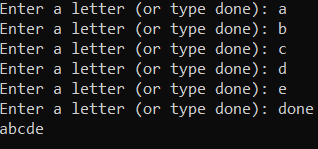
\includegraphics[width = 2.5in]{./imgs/lettersAbcde.PNG} \hfill  
		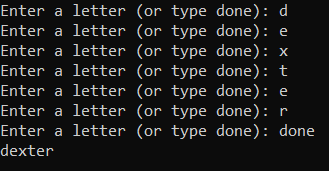
\includegraphics[width = 2.5in]{./imgs/lettersDexter.PNG} \hfill \


%new_question
%%%%%%%%%%%%%%%%%%%%%
	% Problem 6
	% Difficulty: 2
%%%%%%%%%%%%%%%%%%%%%
	\item  
		Write a program that repeatedly asks the user for integers until a negative integer is 
		given. \\ The program should keep track of the sum of the numbers and print the sum at the 
		end \\(not including the negative number).

		For example, \\ \ \hfill
		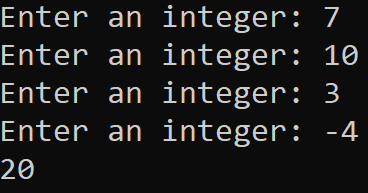
\includegraphics[width = 2.in]{./imgs/AddCalc2.PNG} \hfill  
		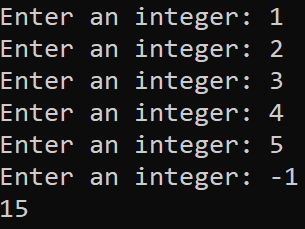
\includegraphics[width = 2.in]{./imgs/AddCalc1.PNG} \hfill \


%new_question
%%%%%%%%%%%%%%%%%%%%%
	% Problem 7
	% Difficulty: 2
%%%%%%%%%%%%%%%%%%%%%
	\item  
		Given a positive integer $n$, the following rules will always create a sequence that 
		ends with 1, called Hailstone Sequence:
		\begin{enumerate}
			\item If $n$ is even, divide by 2
			\item If $n$ is odd, multiply by 3 and add 1 (i.e. $3n+1$)
			\item Continue until $n$ is 1
		\end{enumerate}
		Write a program that prints the hailstone sequence starting at $n=25$.


%new_question
%%%%%%%%%%%%%%%%%%%%%
	% Problem 10
	% Difficulty: 2
%%%%%%%%%%%%%%%%%%%%%
	\item  
		%https://edabit.com/challenge/ksZrMdraPqHjvbaE6
		Write a program that repeatedly asks the user for integers until a negative integer is 
		given.\\  Report back the largest \textbf{even} number the user entered 
		(not including the negative number).  \\
		If the user didn't enter any even numbers report back $-1$.

		For example, \\ \ \hfill
		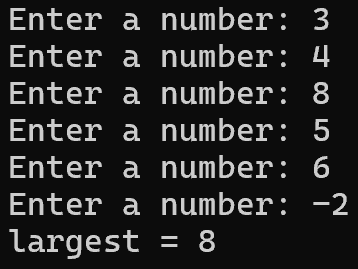
\includegraphics[height = 1.2in]{./imgs/largestEven1.PNG} \hfill  
		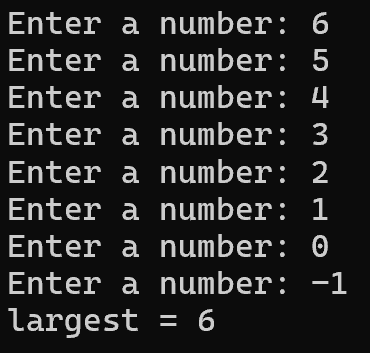
\includegraphics[height = 1.5in]{./imgs/largestEven2.PNG} \hfill  
		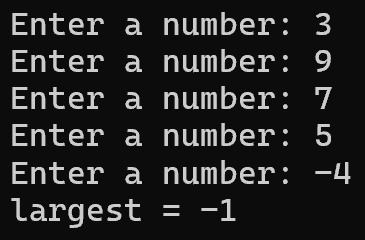
\includegraphics[height = 1.2in]{./imgs/largestEven3.PNG} \hfill \

%end_of_questions

